\documentclass[]{scrartcl}
\usepackage[utf8]{inputenc}
\usepackage[spanish]{babel}
\usepackage{graphicx}
\usepackage{color}
\usepackage[usenames,dvipsnames,svgnames,table]{xcolor}
\usepackage{hyperref}
\usepackage{url}
\usepackage{listings}
\hypersetup{
	colorlinks   = true,
	citecolor    = gray,
	urlcolor     = darkgray,
	linkcolor	 = darkgray
}

%opening
\title{Sistemas Inteligentes para la Gestión en la Empresa\\-\\Práctica 2: Deep Learning para multi-clasificación}
\author{Carlos Cobos Suárez\\Adrián Morente Gabaldón}

\begin{document}

\maketitle
\newpage
\tableofcontents
\newpage

\section{Introducción}

En este proyecto vamos a realizar diversas aproximaciones al tratamiento de técnicas de \textbf{aprendizaje profundo} con el lenguaje \textbf{\textit{R}}. Tras ponernos en situación con los fundamentos teóricos necesarios para entender el desarrollo realizado, comentaremos las soluciones pensadas y las que finalmente se hayan implementado; realizando después una discusión de los resultados obtenidos.\\

El conjunto de datos (o \textit{dataset}) que utilizaremos se corresponde con el de \textbf{\textit{PetFinder.my Adoption Prediction}}, y podemos encontrarlo en la plataforma \href{https://kaggle.com}{Kaggle} \cite{petfinder-dataset}. Los datos contenidos clasifican un histórico de perros y gatos alojados en centros de adopción de animales, con diversas características y almacenando el \textbf{tiempo de adopción} de cada una de estas mascotas.\\

El trabajo a desarrollar en este proyecto versa sobre el \textbf{entrenamiento de modelos de predicción} que, a partir de imágenes o de un conjunto de características de animales, clasifiquen éstos por tiempo de adopción. Para dicha clasificación, utilizaremos \textbf{cinco categorías} (las cuales se ordenan según el tiempo de adopción en orden ascendente). Lógicamente, la finalidad del trabajo será la de obtener la mejor precisión general posible, para lo que utilizaremos distintos modelos basados en \textbf{aprendizaje profundo}.\\

Dado que para el entrenamiento se dispone de un gran conjunto de datos ya clasificado, realizaremos algún \textbf{histograma}, lo que trata de un gráfico de barras que muestra el cardinal del conjunto de datos de cada una de las distintas categorías mencionadas.\\

Por otro lado, realizaremos también un \textbf{trabajo de investigación} relacionado con la aplicación de \textbf{técnicas de binarización}, planteando un marco teórico y comentando las distintas posibilidades que ofrecen.

\section{Fundamentos teóricos}

	Para entender tanto la finalidad del proyecto como los pasos realizados para su compleción, debemos ubicarnos en un marco teórico apropiado. Para empezar, antes de abordar la temática relacionada con el \textbf{aprendizaje profundo}, debemos hablar del \textbf{aprendizaje automático} y las técnicas más destacadas para su puesta en uso, como pueden ser las \textbf{redes neuronales} de diversos tipos.
	
	\subsection{Redes neuronales}
	
		Sabemos que la unidad básica de una red neuronal es, lógicamente, la \textbf{neurona}; cuya función es recibir unos datos de entrada, procesarlos mediante algunas operaciones matemáticas, y producir una salida.\\
		
		Estas entradas pueden provenir de la entrada al sistema o de la salida por parte de otras neuronas. Además, el número de éstas es variable, como podemos ver en la figura \ref{neuron}, donde se visualiza un ejemplo de neurona con dos entradas y una salida \cite{introduction-neural-networks}.\\
	
		\begin{figure}[h]
			\centering
			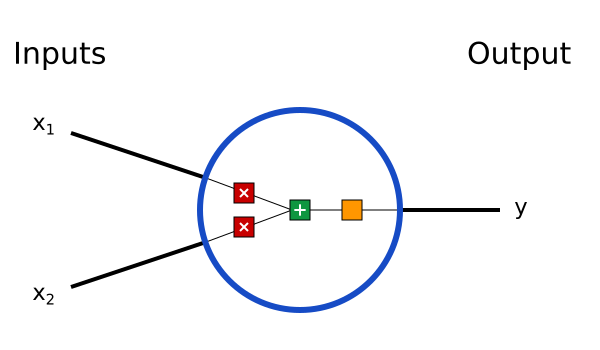
\includegraphics[width=0.5\textwidth]{./img/neuron}
			\caption{Neurona simple con dos entradas y una salida.}
			\label{neuron}
		\end{figure}
	
		Como se podría esperar a raíz de su nombre, sabiendo lo que es una neurona, podemos esperar que una \textbf{red neuronal} sea un conjunto conectado de varias neuronas. Podemos ver un ejemplo en la figura \ref{neural-network}.\\
		
		\begin{figure}[h]
			\centering
			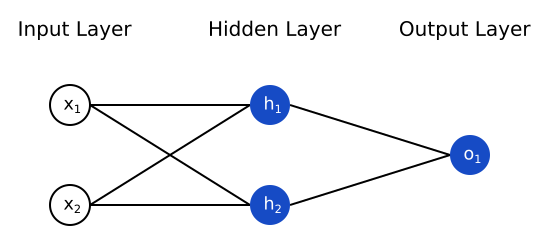
\includegraphics[width=0.5\textwidth]{./img/neural-network}
			\caption{Red neuronal simple con dos entradas y una salida.}
			\label{neural-network}
		\end{figure}
	
		Como podemos observar en dicha figura \ref{neural-network}, la red consta de una capa de entrada con dos neuronas, una red intermedia con otras dos, y finalmente de la capa de salida. Debemos saber que en dicha capa intermedia es donde se realizan sobre los datos de entrada todas las operaciones matemáticas que comentábamos anteriormente.\\
		
		Finalmente, en la capa de salida se combinan como entradas las salidas de la capa intermedia para, mediante una \textbf{función de activación}, producir una determinada salida.
		
	\subsection{Redes neuronales para tratamiento de imágenes}
	
		Conociendo las redes neuronales simples, debemos saber que \textbf{no son apropiadas para su uso con imágenes} debido a lo siguiente \cite{intro-convolutional-nn}:
		
		\subsubsection*{Tamaño de las imágenes}
		
			Los píxeles de una imagen son los que han de introducirse como entradas a la primera capa de una red neuronal. Si una imagen consta de 150 píxeles en blanco y negro, existirán 150 entradas. Si la imagen es a color (en modo \textit{RGB}), el número de entradas se multiplican por los tres canales de dicho formato.\\
			 
			Esto quiere decir que si una imagen consta de millones de píxeles, como encontramos actualmente en las tomadas por un teléfono móvil cualquiera, tendríamos que entrenar \textbf{millones de pesos} en la primera capa, lo que es prácticamente imposible en cualquier ordenador del que dispongamos.
			 
		\subsubsection*{Posición de las imágenes}
		
			Aunque en dos imágenes se muestre el mismo objeto para cuya detección ha sido entrenada la red neuronal simple, con una de este tipo no se es capaz de detectar que dicho objeto pueda cambiar en el espacio mostrado por la imagen. Es decir, aunque aparezca la misma cara humana que en otra imagen antes estudiada, que este elemento cambie de posición en la imagen implica que no sean las mismas neuronas las que se activen, por lo que el resultado de salida puede (y con mucha probabilidad) no ser el esperado.
			
		\subsubsection*{Solución}
		
			La solución para estos problemas la encontramos en las \textbf{redes neuronales de tipo convolucional}, que no son más que redes simples como las ya estudiadas pero que utilizan unas capas especiales, llamadas \textit{convolucionales}.\\
			
			Una \textbf{convolución} no es más que un filtro aplicado de forma iterativa a la imagen en forma de pequeña matriz de dos dimensiones. Un ejemplo práctico lo podemos ver en la referencia \cite{intro-convolutional-nn}, que aplica un \textbf{filtro horizontal de \textit{Sobel}} para mostrar la detección de límites en una imagen.\\
			
			En este caso el filtro usado (o \textit{kernel}) se muestra en la figura \ref{conv-filter}. Adicionalmente, en la figura \ref{conv-filter-result} se visualizan a la izquierda la imagen original sobre la que se aplica el filtro, y a su derecha la imagen resultante. Como podemos ver, el resultado es una nueva fotografía en blanco y negro donde se manifiestan los límites más relevantes de dicha foto.\\
			
			\begin{figure}[h]
				\centering
				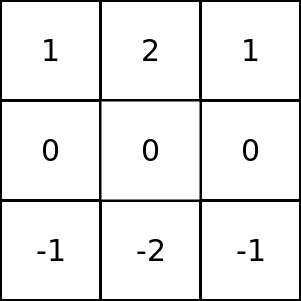
\includegraphics[width=0.2\textwidth]{./img/horizontal-sobel}
				\caption{Ejemplo de matriz de convolución - Filtro horizontal de \textit{Sobel}.}
				\label{conv-filter}
			\end{figure}
		
			\begin{figure}[h]
				\centering
				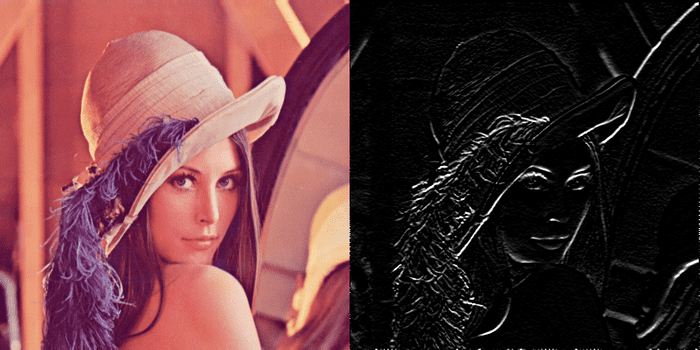
\includegraphics[width=0.6\textwidth]{./img/lenna+horizontal}
				\caption{Imagen original y su resultante tras aplicar el filtro convolucional de \textit{Sobel}.}
				\label{conv-filter-result}
			\end{figure}
		
			Utilizando la detección de límites de forma previa al entrenamiento de la red, se delimitan mucho mejor los elementos contenidos en la imagen, por lo que se favorece mucho dicha fase de aprendizaje.
	
	\subsection{\textit{Deep Learning}}
	
		Se conoce como \textbf{aprendizaje profundo} al campo de aplicación del \textbf{aprendizaje automático} donde se hace un uso más extenso de técnicas basadas en \textbf{redes neuronales artificiales}. Estas redes utilizadas son capaces de aprender \textit{profundamente} para trabajar con problemas como reconocimiento de imágenes, de texto o de voz; además de otras aplicaciones como filtrado colaborativo en redes sociales y visión por computador.\\
		
		La diferencia principal entre una red neuronal simple y las redes de \textit{aprendizaje profundo} reside en que las primeras, como ya hemos visto anteriormente, contienen una suma de tres capas: la de \textbf{entrada}, la \textbf{intermedia} (donde se aplican las operaciones) y la de \textbf{salida}.\\
		
		Por otro lado, en las redes neuronales de \textit{deep learning} el número de capas intermedias es mayor, con lo que se consigue un mejor aprendizaje. Esto se debe a que el número de neuronas (y por tanto de pesos en el modelo final) es mayor; y cuanto más alto sea el número de hiperparámetros presentes en un algoritmo, mayor es la capacidad de entrenamiento que tendrá dicho modelo final.
		
		\begin{figure}[h]
			\centering
			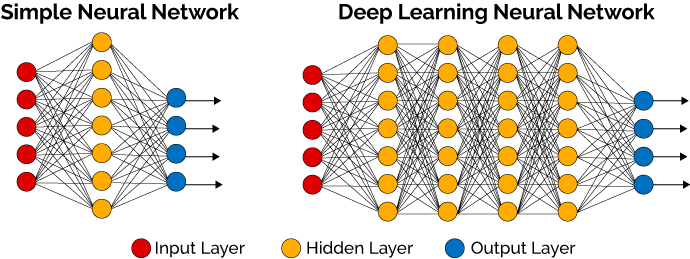
\includegraphics[width=0.8\textwidth]{./img/neural-network-differences}
			\caption{Diferencia entre red neuronal simple y red de aprendizaje profundo.}
			\label{nn-differences}
		\end{figure}
	
		las clasificaciones multicategóricas fallan porque no suelen detectar muy bien las clases. esto se puede resolver si nos llevamos ese mismo problema a varios más sencillos de clasificación binaria, obteniendo así más clasificadores.
	
		\subsubsection{Técnicas de binarización}
		
		\subsubsection{\textit{Ensembles}}
		
			forma de juntar todos los clasificadores binarios para tener un solo modelo final.

\section{Descripción de las redes empleadas}

	\subsection{Primera aproximación - Red vista en clase}
	
	\subsection{Segunda aproximación - Balanceo de clases}
	
	funciona con pesos. como tenemos los datos del histograma, podemos sacar los porcentajes (pesos) a utilizar para que estén balanceados con el resto de clases.
	
	\subsection{Tercera aproximación - \textit{Data augmentation}}
	
\section{Discusión de resultados}

\section{Conclusiones}

\bibliographystyle{plain}
\bibliography{sources}

\end{document}
